\documentclass[10pt]{article}
\usepackage[utf8]{inputenc}
\usepackage[spanish]{babel}
\usepackage{amsmath}
\usepackage{amsfonts}
\usepackage{amssymb}
\usepackage{graphics}
\usepackage{graphicx}
\usepackage[left=2cm,right=2cm,top=2cm,bottom=2cm]{geometry}
\usepackage{imakeidx}
\makeindex[columns=3, title=Alphabetical Index, intoc]
\usepackage{listings}
\usepackage{xcolor}
\usepackage{multicol}
\usepackage{changepage}
\usepackage{float}
\usepackage{cite}
\usepackage{url}
\usepackage{hyperref}
\usepackage[document]{ragged2e}
\hypersetup{
    colorlinks=true,
    linkcolor=blue,
    filecolor=magenta,
    urlcolor=blue,
}

\definecolor{codegreen}{rgb}{0,0.6,0}
\definecolor{codegray}{rgb}{0.5,0.5,0.5}
\definecolor{codepurple}{rgb}{0.58,0,0.82}
\definecolor{backcolour}{rgb}{0.95,0.95,0.92}

\lstdefinestyle{mystyle}{
    backgroundcolor=\color{backcolour},
    commentstyle=\color{codegreen},
    keywordstyle=\color{magenta},
    numberstyle=\tiny\color{codegray},
    stringstyle=\color{codepurple},
    basicstyle=\ttfamily\footnotesize,
    breakatwhitespace=false,
    breaklines=true,
    captionpos=b,
    keepspaces=true,
    numbers=left,
    numbersep=5pt,
    showspaces=false,
    showstringspaces=false,
    showtabs=false,
    tabsize=3
}

\lstset{style=mystyle}

\title{Centro de Investigación en Cómputo\\Instituto Politécnico Nacional\\Metaheurísticas\\Actividad No. 7\\ Solución de problemas mediante Recocido Simulado\\Curso impartido por: Dra Yenny Villuendas Rey}

\author{Adrian González Pardo}

\date{21 de octubre de 2020}

\newcommand\tab[1][1cm]{\hspace*{#1}}

\begin{document}
\maketitle
\section{Recocido Simulado (Simulated Annealing, SA)}
\begin{center}
  \begin{tabular}{|p{6cm}|p{6cm}|}
    \hline
    Ventajas & Desventajas \\
    \hline
    Permite obtener una solución aproximada al minimo global & Puede llegar a pasar que en la siguiente iteración a la solución salga del minimo global y este se alcance un resultado minimo local \\
    \hline
    Permite encontrar soluciones razonables (En tiempo) & La solución encontrada puede no ser la mejor\\
    \hline
    Utiliza poca memoria & No permite vuelta atras en más de 1 paso\\
    \hline
  \end{tabular}
\end{center}
\section{Pseudocódigo SA}
\lstinputlisting[language=Ruby]{./pseudo.rb}
\section{SA vs RMHC}
La diferencia más notable entre estos dos algoritmos, es notablemente que el RMHC se basa en la mutación aleatoria de un conjunto de datos, generando un camino de solución del arbol de soluciones, mientras que SA parte de una solución donde el mismo algoritmo esta bioinspirado en un proceso físico que busca un ablandamiento para la formación o moldeo de estructuras de metal, entonces si bien ambos son algoritmos heurísticos RMHC se aplica en problemas cuya solución puede ser mutada y en este caso no puede salir de un mínimo local si este cae en ese espacio, mientras que SA permite admitir una respuesta no optima para seguir explorando el espacio de soluciones.
\section{Investigación de los ultimos 3 años aplicando el algoritmo de SA}
\begin{enumerate}
  \item Agosto de 2020. Diseño del controlador de regulación automática de voltaje usando SA hibrido con algoritmos de optimización de Forrajeo de mantarraya. \underline{\href{https://www.sciencedirect.com/science/article/pii/S2090447920301416}{Paper}}
  \item Enero de 2020. Una nueva técnica híbrida de programación genética basada en SA para predecir la capacidad de carga máxima de las pilas. \underline{\href{https://link.springer.com/article/10.1007/s00366-019-00932-9}{Paper}}
  \item Junio de 2018. Optimización de SA evolutivo multiobjetivo para el equilibrado de la línea de desmontaje multirrobótico de modelo mixto con tiempo de procesamiento de intervalo. \underline{\href{https://www.tandfonline.com/doi/abs/10.1080/00207543.2019.1602290}{Paper}}
\end{enumerate}
\section{Aplicaciones SA}
\subsection{Knapsack}
Modelación Matemática\\
Sean dos funciones
\[f(x)=\sum_{i=1}^{N}x^{I}_{i}h(x_{i})\]
\[g(x)=\sum_{i=1}^{N}x^{I}_{i}p(x_{i})\;<=\;peso\_maximo\]
Donde:\\
\(\displaystyle X\;es\;un\;vector\;de\;la\;forma\;X=(x_{1},x_{2},\cdots,x_{N})\)\\\vspace{0.25cm}
\(\displaystyle X^{I}\;es\;un\;vector\;el\;cual\;es\;parecido\;a\;X\;pero\;sus\;valores\;x_{i}^{I}\in[0,1]\;y\;x_{i}^{I}\in\mathbb{Z}\)\\\vspace{0.25cm}
\(\displaystyle h(x)\;es\;una\;funci\acute{o}n\;la\;cual\;devuelve\;el\;beneficio\;total\;de\;los\;objetos\;x_{i}\;en\;la\;mochila\)\\\vspace{0.25cm}
\(\displaystyle p(x)\;es\;una\;funci\acute{o}n\;la\;cual\;devuelve\;el\;peso\;total\;de\;los\;objetos\;x_{i}\;en\;la\;mochila\)\\\vspace{0.25cm}
En el cual el algoritmo de SA busca iterar sobre cada contenido o casilla del vector $X^{I}$ de tal forma que se obtiene una solución y sobre esta se busca encontrar una mejor solución.\\
Por lo cual el test objetivo del algoritmo es encontrar el optimo global sin que este pueda caer en el optimo local o en otra zona.
\subsection{Travel Salesman Problem TSP}
Modelación Matemática\\
Sea la función
\[f(x)=\sum_{i=1}^{N}\sum_{j=1}^{N}x^{I}_{i,j}g(x_{i,j})\]
Donde:\\
\(\displaystyle X\;es\;una\;matriz\;de\;NxN\;la\;cual\;trabajara\;para\;obtener\;el\;costo\;con\;la\;funci\acute{o}n\;g(x)\)\\\vspace{0.25cm}
\(\displaystyle X^{I}\;es\;una\;matriz\;de\;NxN\;la\;cual\;contiene\;valores\;que\;permiten\;saber\;si\;el\;nodo\;es\;considerado\;o\;no\;para\;la\;soluci\acute{o}n\;\)\\\vspace{0.25cm}
\(\displaystyle La\;notaci\acute{o}n\;(i,j)\;significa\;\;i\;como\;nodo\;origen\;que\;va\;a\;j\)\\\vspace{0.25cm}
\(\displaystyle x^{I}_{i,j}\;es\;un\;valor\;de\;la\;matriz,\;donde\;x^{I}_{i,j}\in[0,1]\;y\;x_{i,j}\in\mathbb{Z}\)\\\vspace{0.25cm}
\(\displaystyle Si\;x_{i,j}=-1\;significa\;que\;no\;hay\;una\;conexi\acute{o}n\;de\;i\;a\;j\)\\\vspace{0.25cm}
\(\displaystyle g(x)\;es\;una\;funci\acute{o}n\;la\;cual\;devuelve\;el\;valor\;costo\;de\;ir\;de\;i\;a\;j\)\\\vspace{0.25cm}
De tal forma que este algoritmo de SA busca iterar sobre el contenido de una solución cualquiera y sobre cada vertice que este modifique el algoritmo buscara realizar una operación de intercambio de la forma $x_{i,j}$ cambia con $x_{j,i}$ de tal forma que el movimiento sea valido y este modifique la solución.\\
El test objetivo de esta solucion es encontrar una solución de minimización de costo de tal forma que la solución recorra todos los nodos.
\subsection{Función de Minimización en D dimensiones}
Modelación Matemática\\
Sea la función
\[f(x)=\sum_{i=1}^{N}x_{i}^{2}\]
Donde:\\
\(\displaystyle x_{i}\in\mathbb{R}\)\\\vspace{0.25cm}Descrito en los intervalos \(\displaystyle x_{i}\in[-10,10]\)\\\vspace{0.25cm}
Donde sabemos que los puntos minimos de cada $x_{i}$ los encontramos cuando el valor asignado a el es $x_{i}=0$ por lo tanto el ir variando los valores para que el programa se acerque hacia $0$\\
De tal manera que el algoritmo de SA seleccionara 1 indice en el cual se le asignara un valor a $x_{i}$.\\
En el test objetivo es encontrar 1 punto aproximado en el que la función se aproxime a $0$ o en el que al menos una coordenada $x_{i}\sim 0$
\section{Ejecución a mano.}
\subsection{Knapsack}
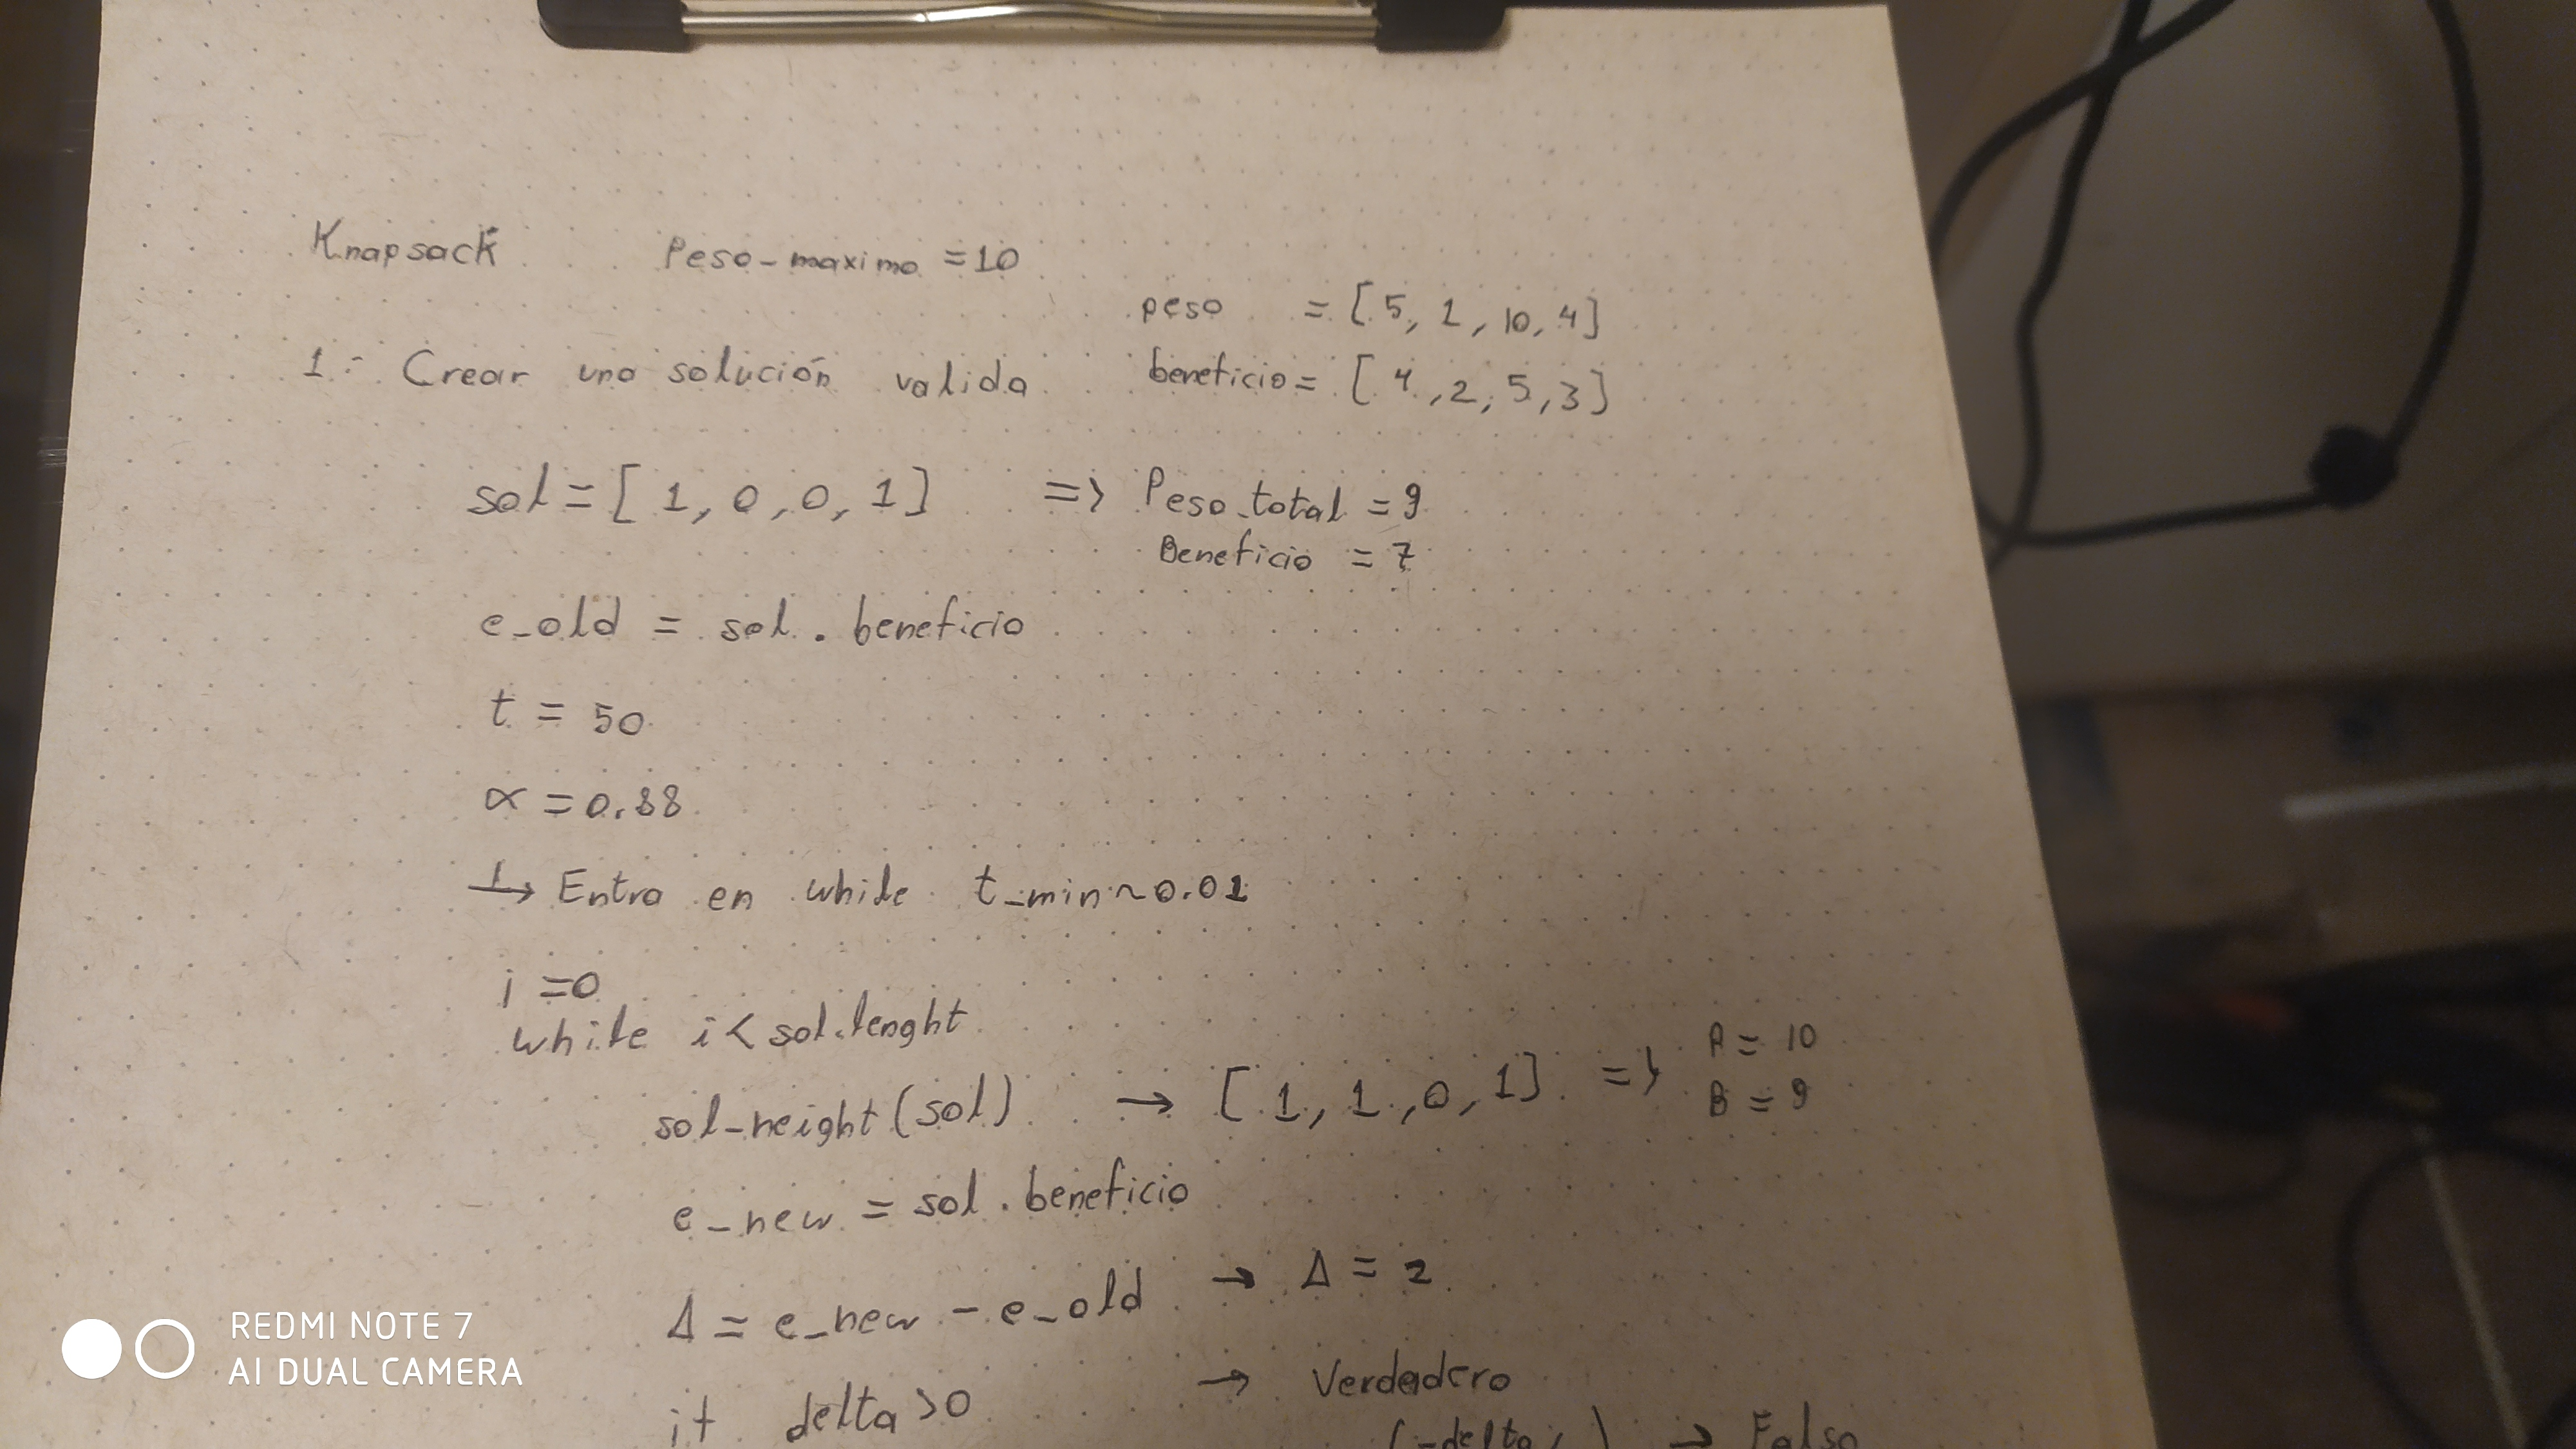
\includegraphics[scale=0.135]{imgs/k-1.jpg}\\
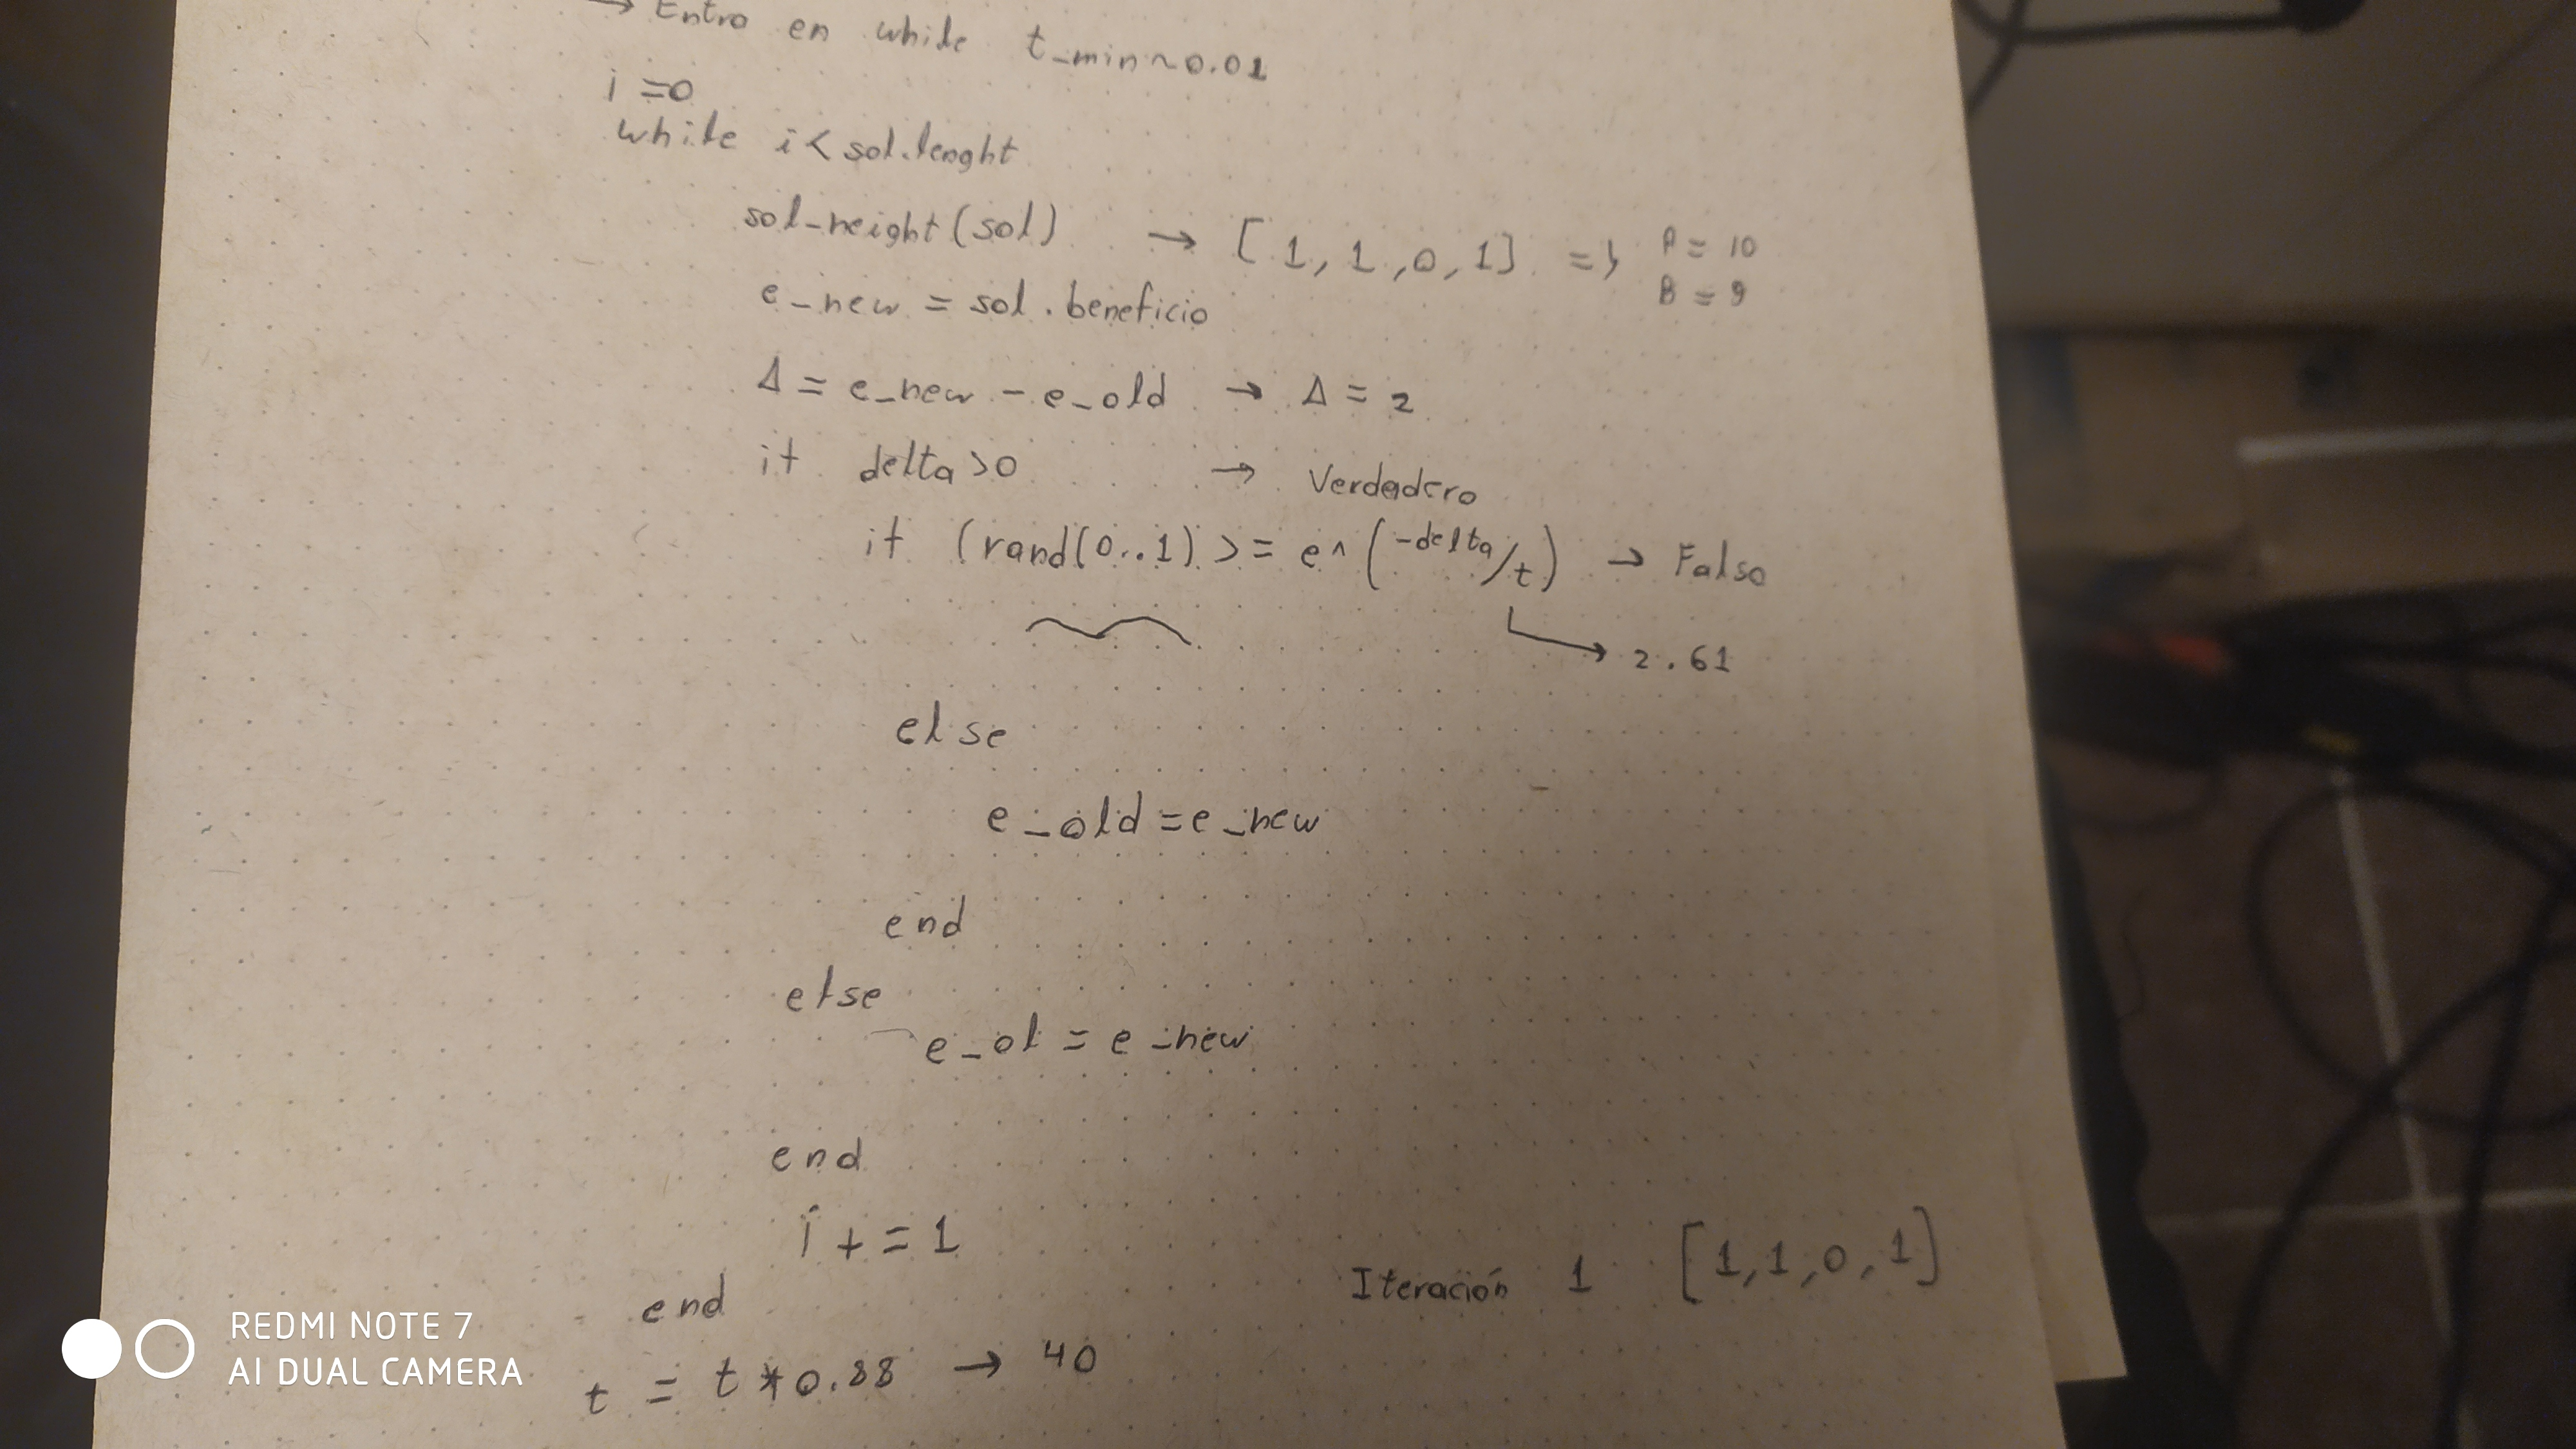
\includegraphics[scale=0.135]{imgs/k-2.jpg}
\subsection{TSP}
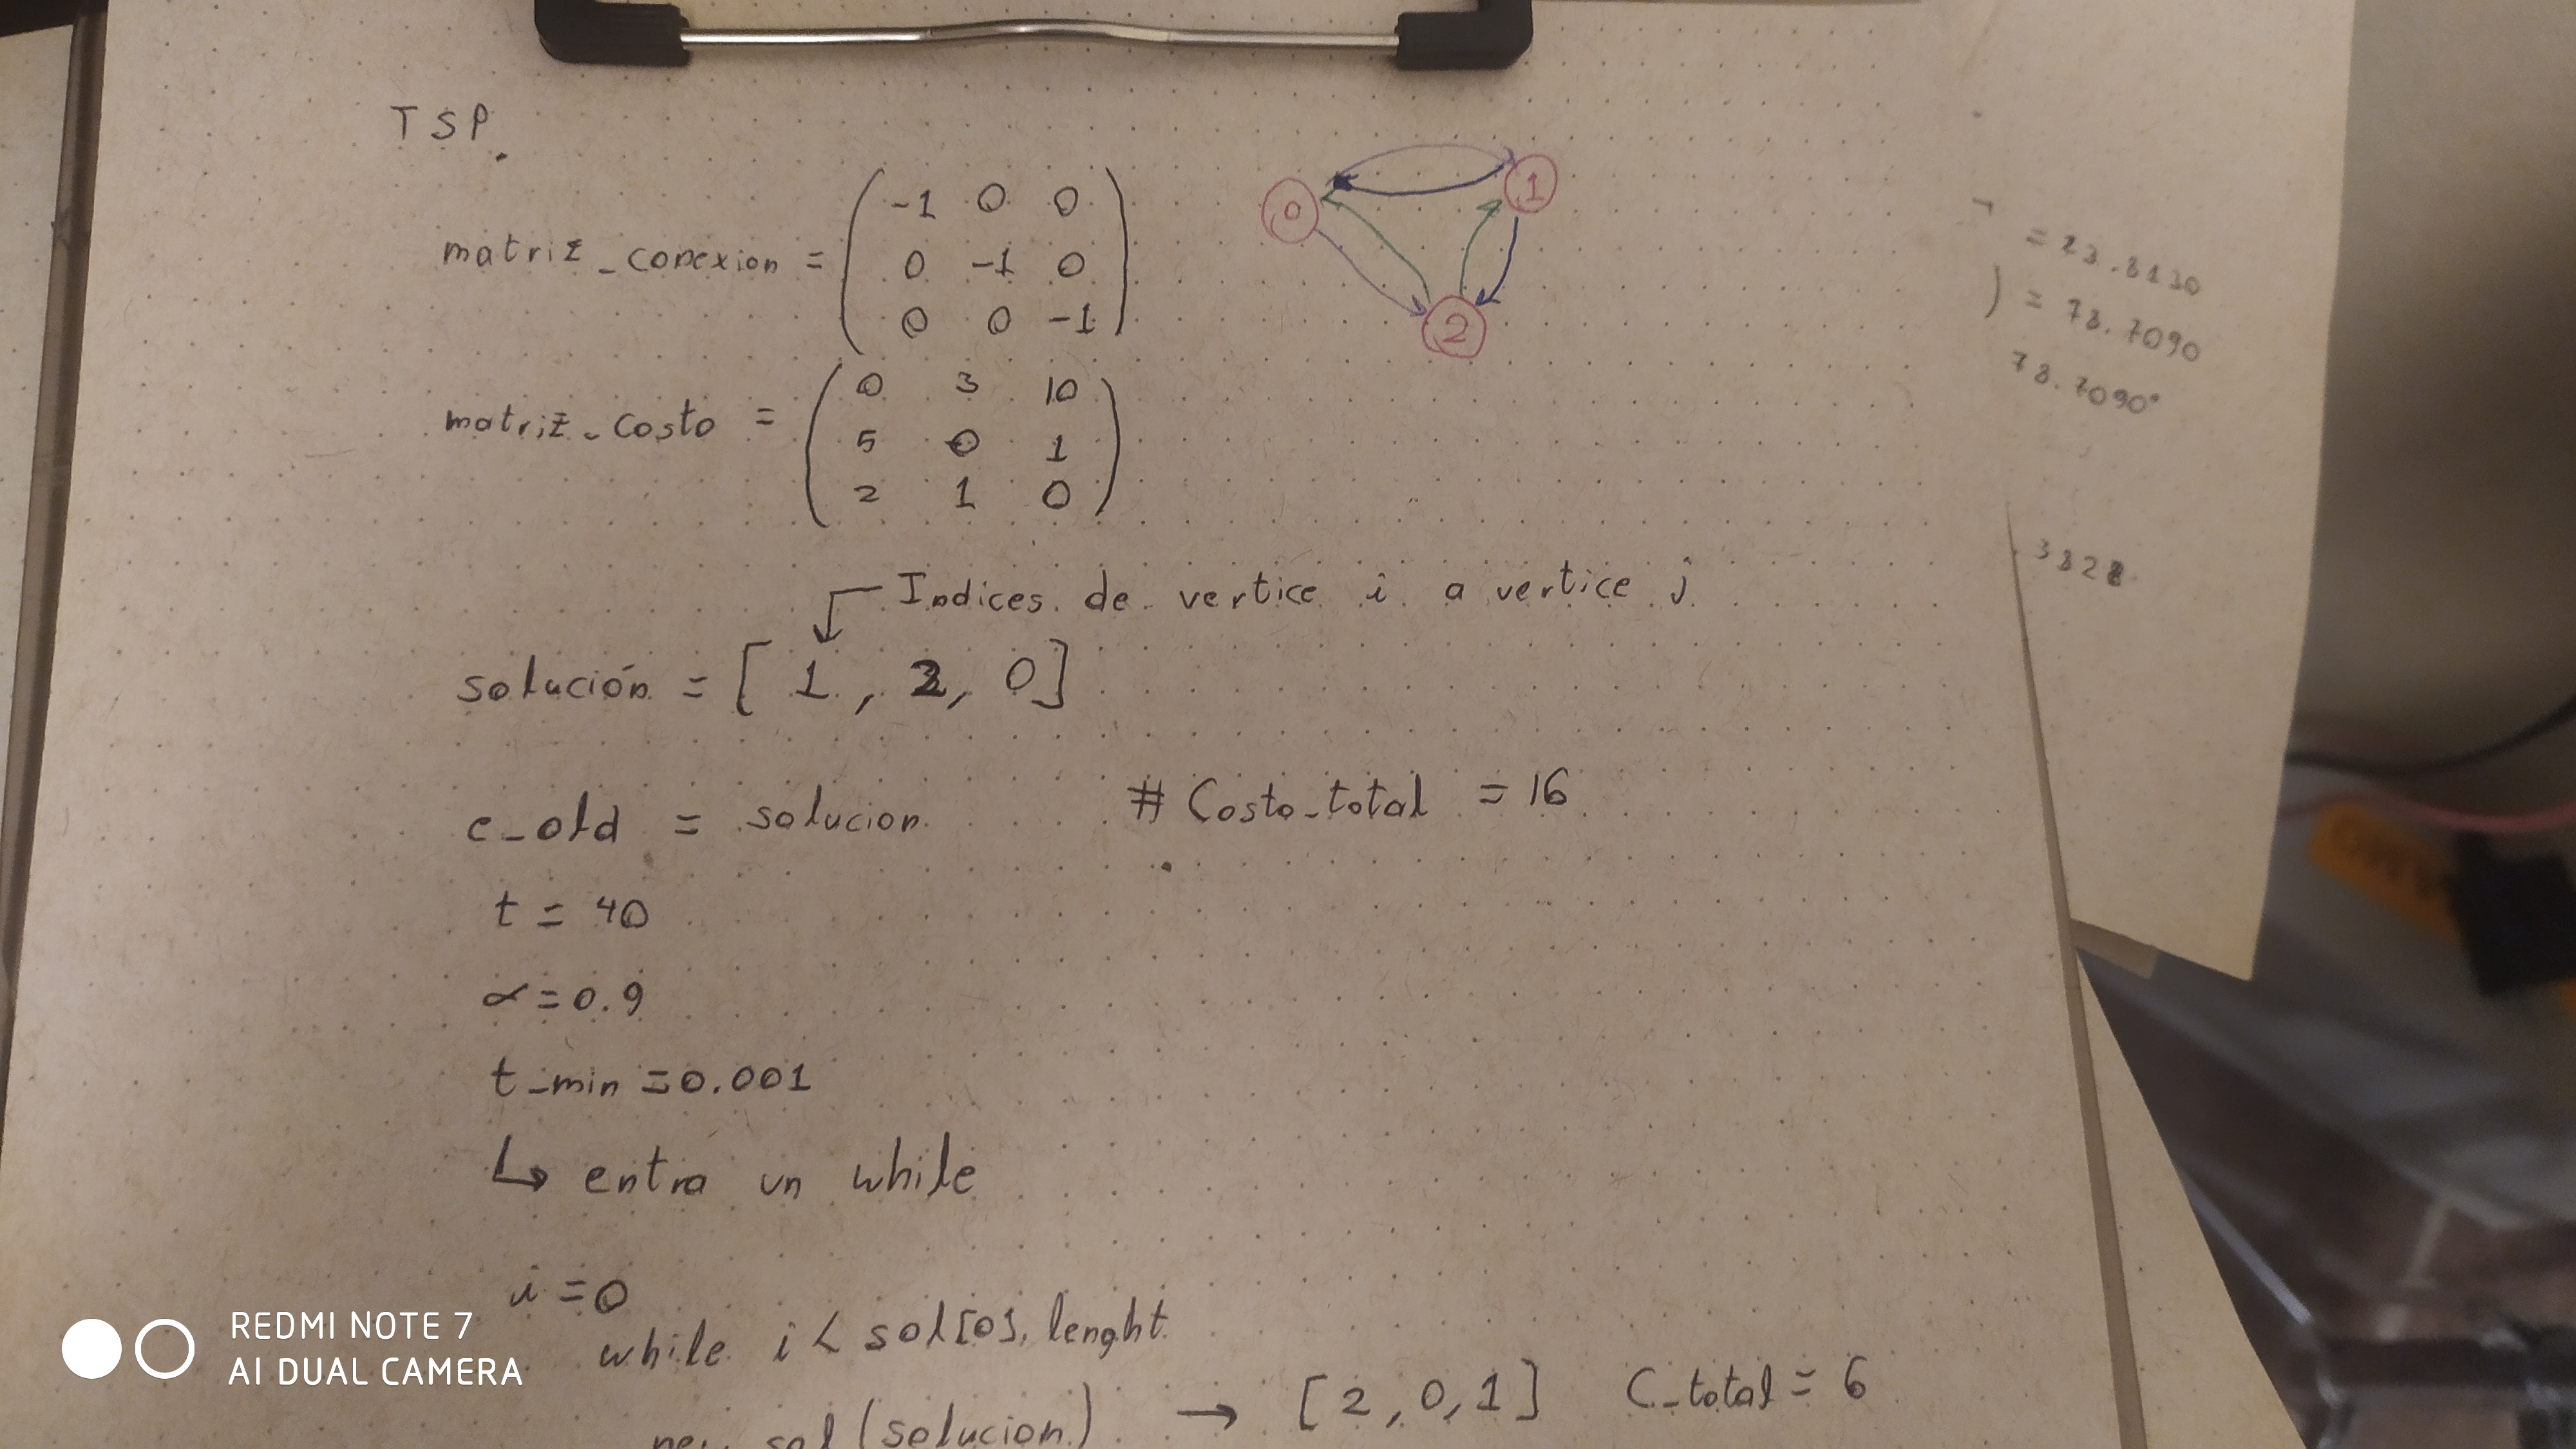
\includegraphics[scale=0.135]{imgs/tsp-1.jpg}\\
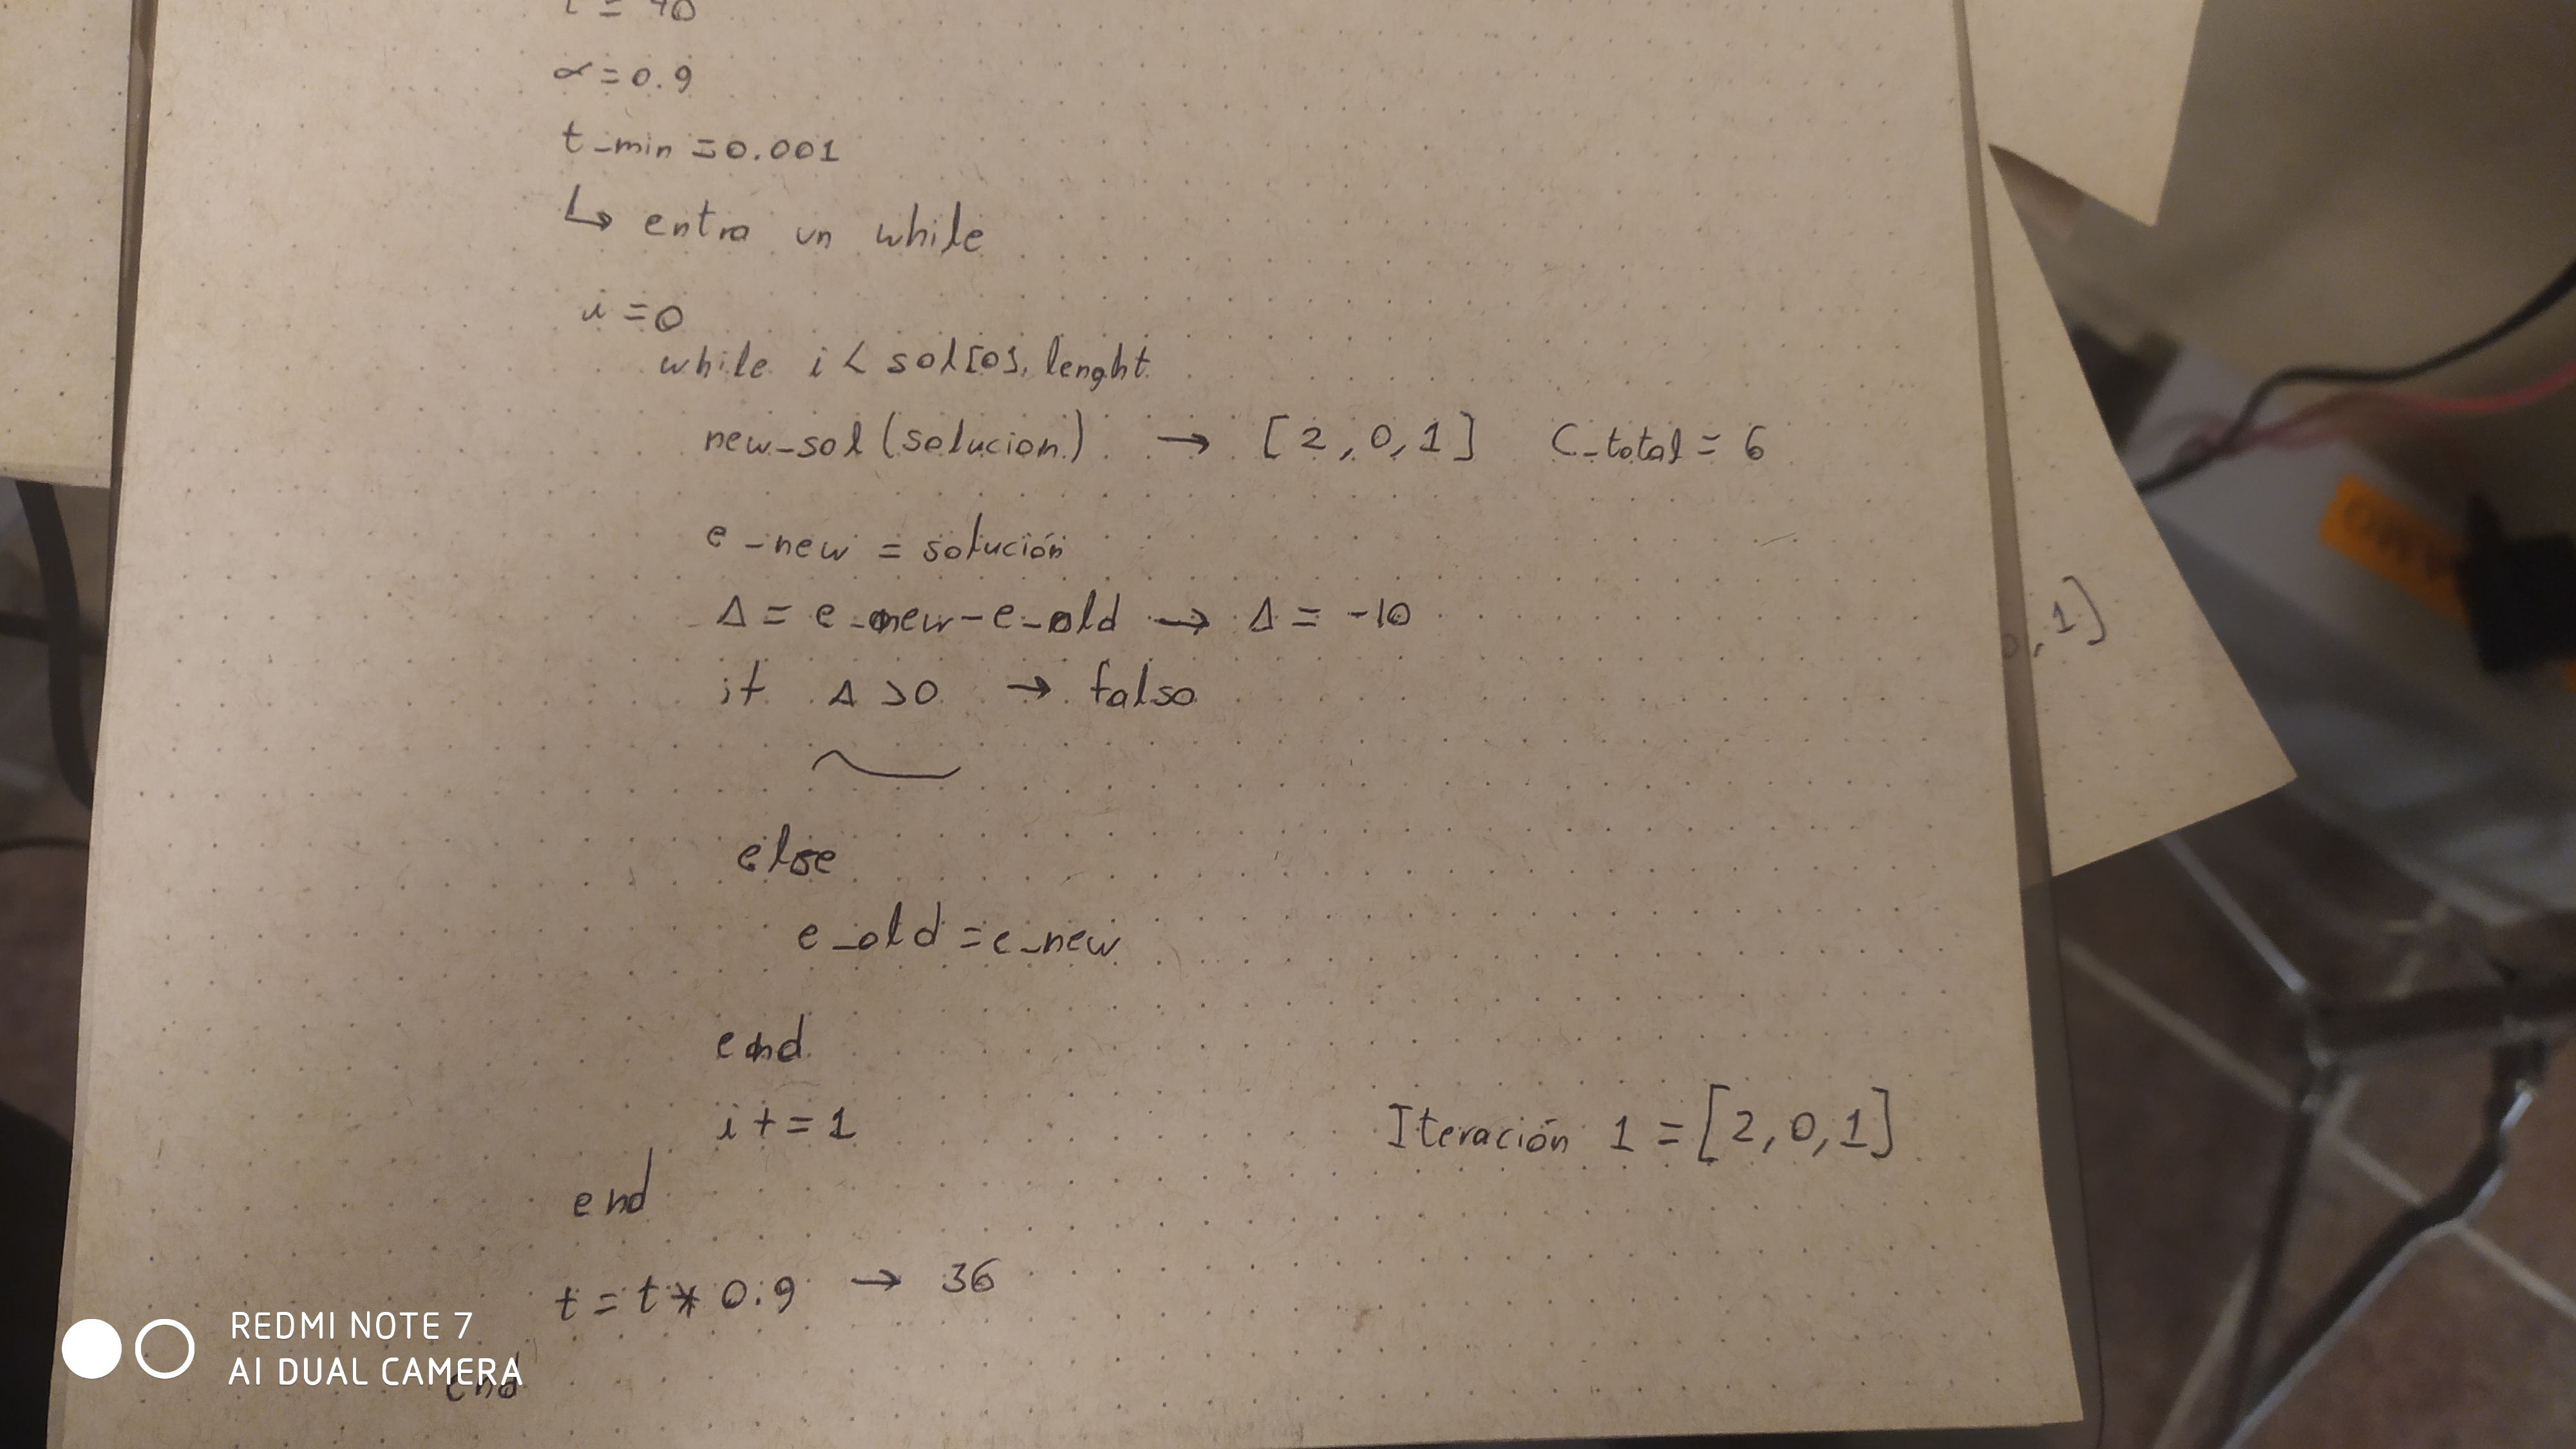
\includegraphics[scale=0.135]{imgs/tsp-2.jpg}
\subsection{Función de Minimización en D dimensiones}
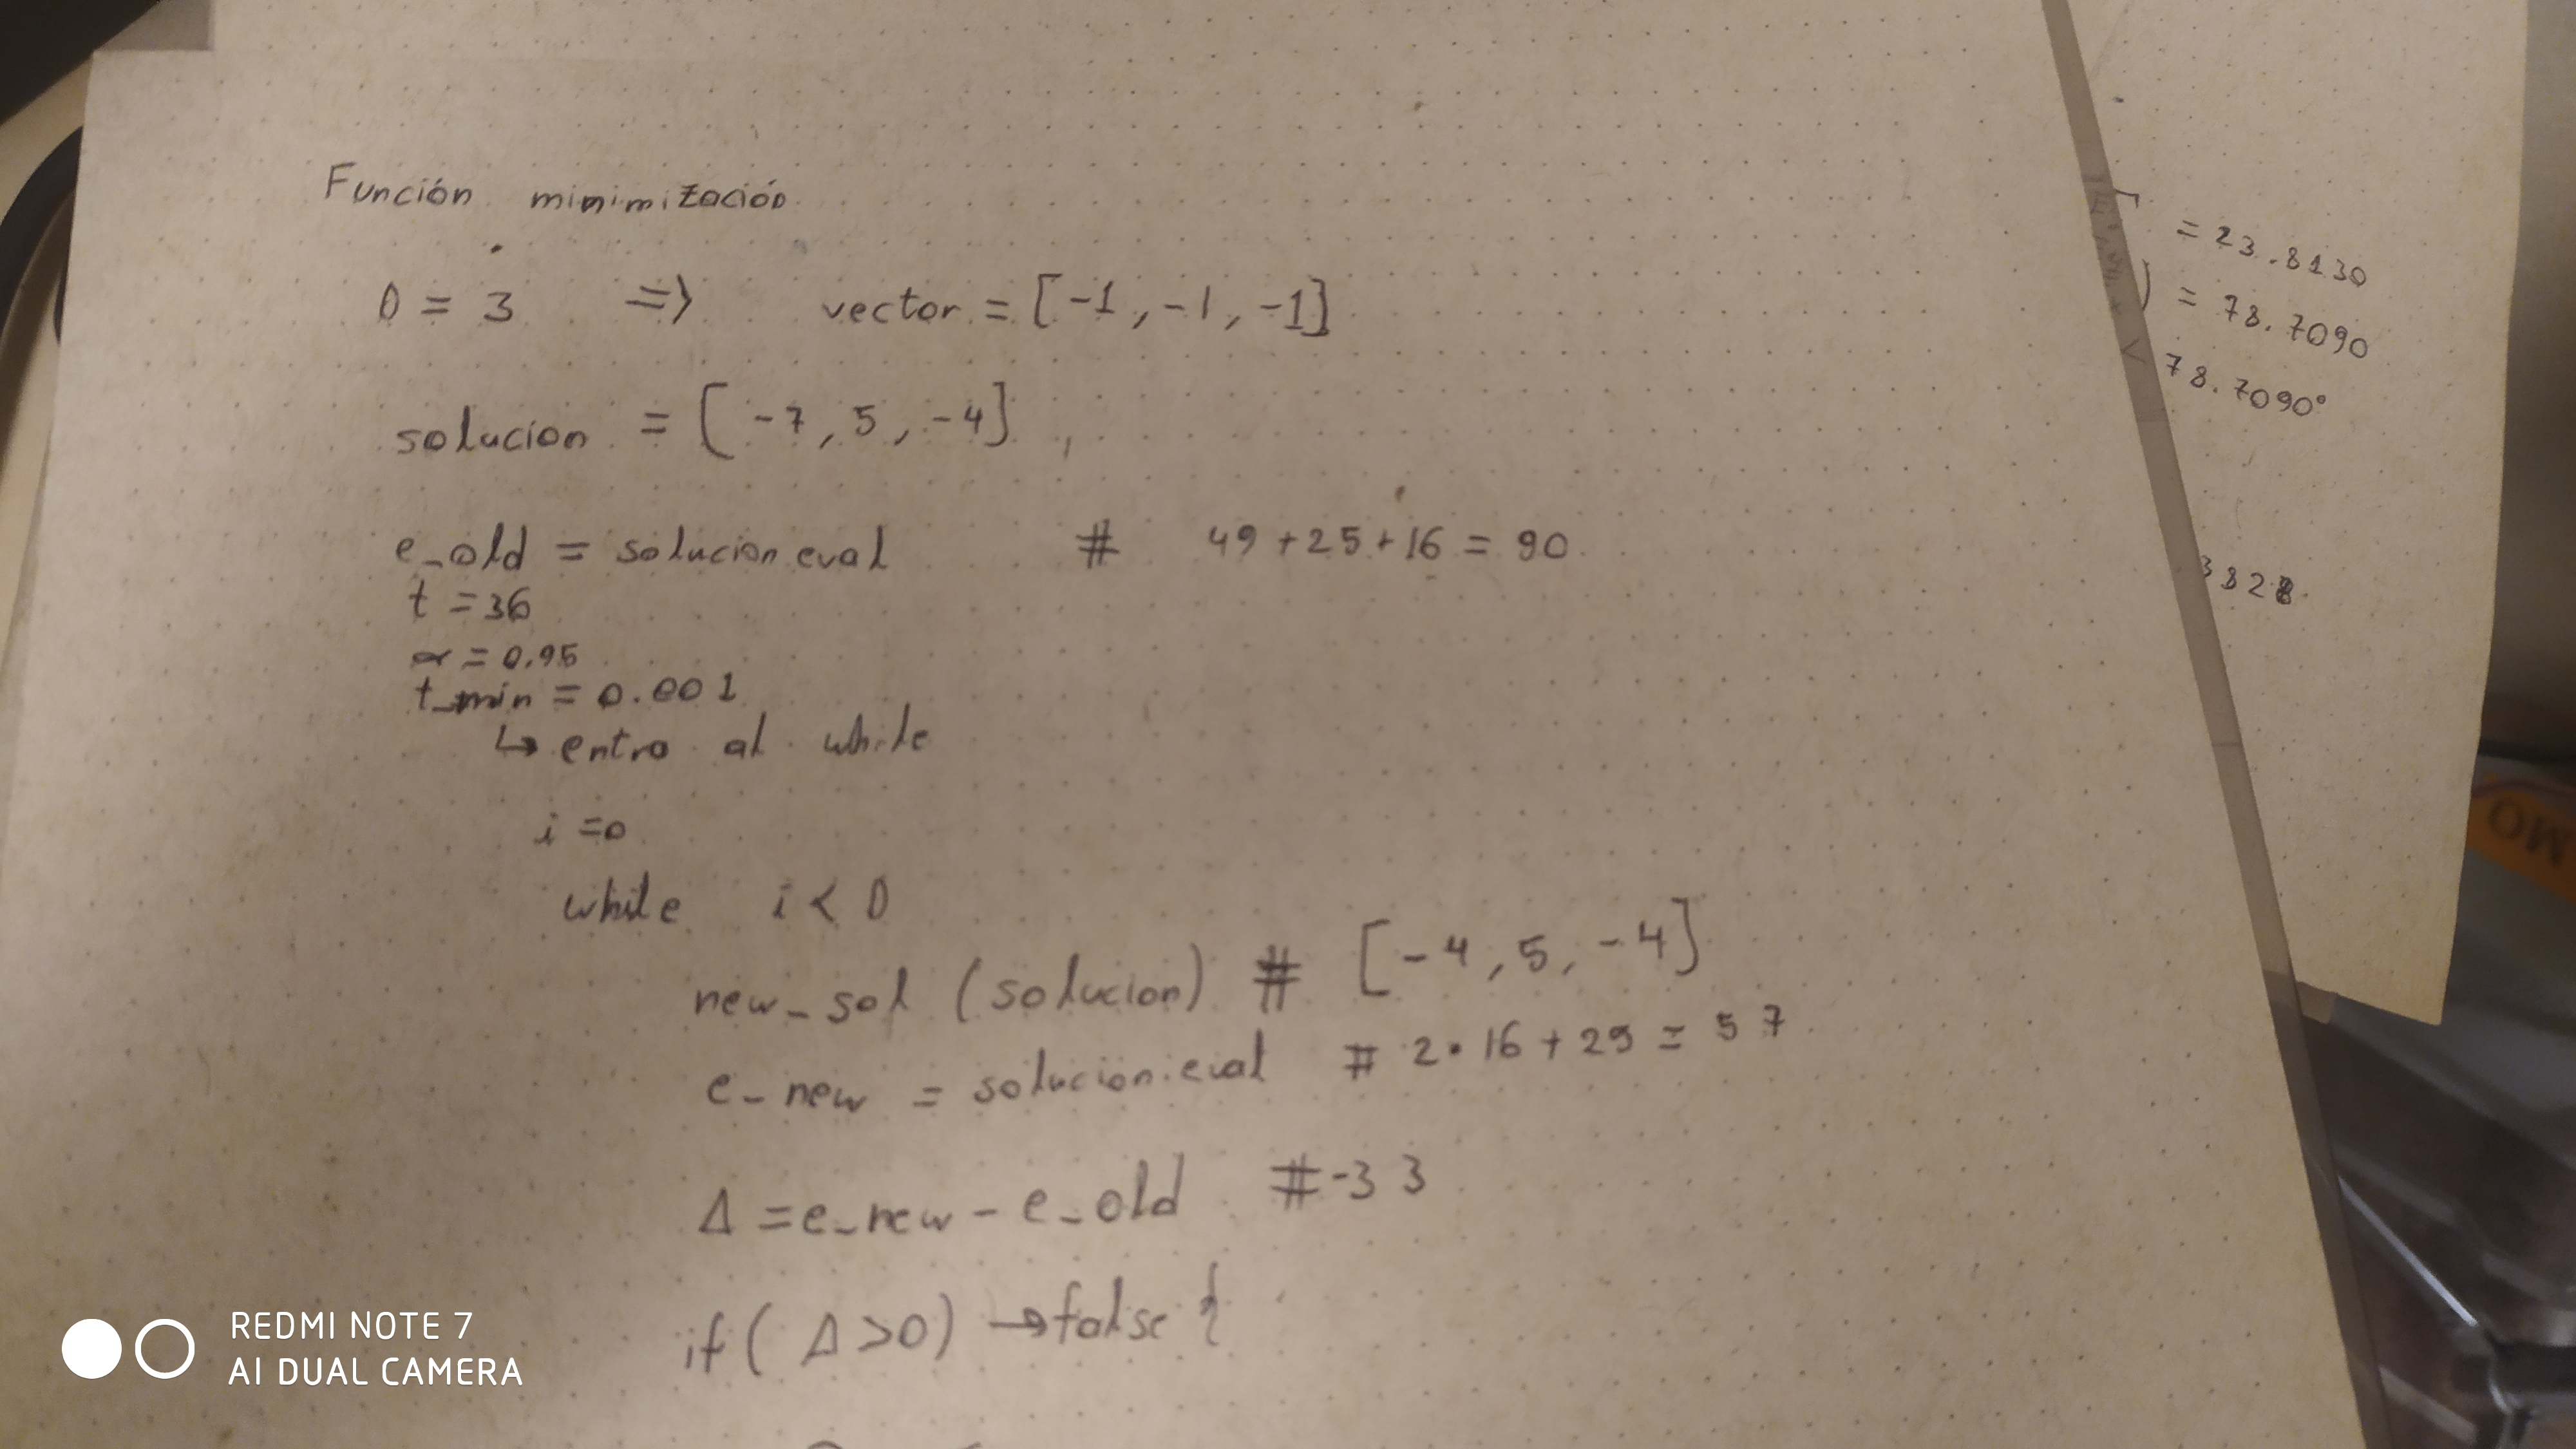
\includegraphics[scale=0.135]{imgs/min-1.jpg}\\
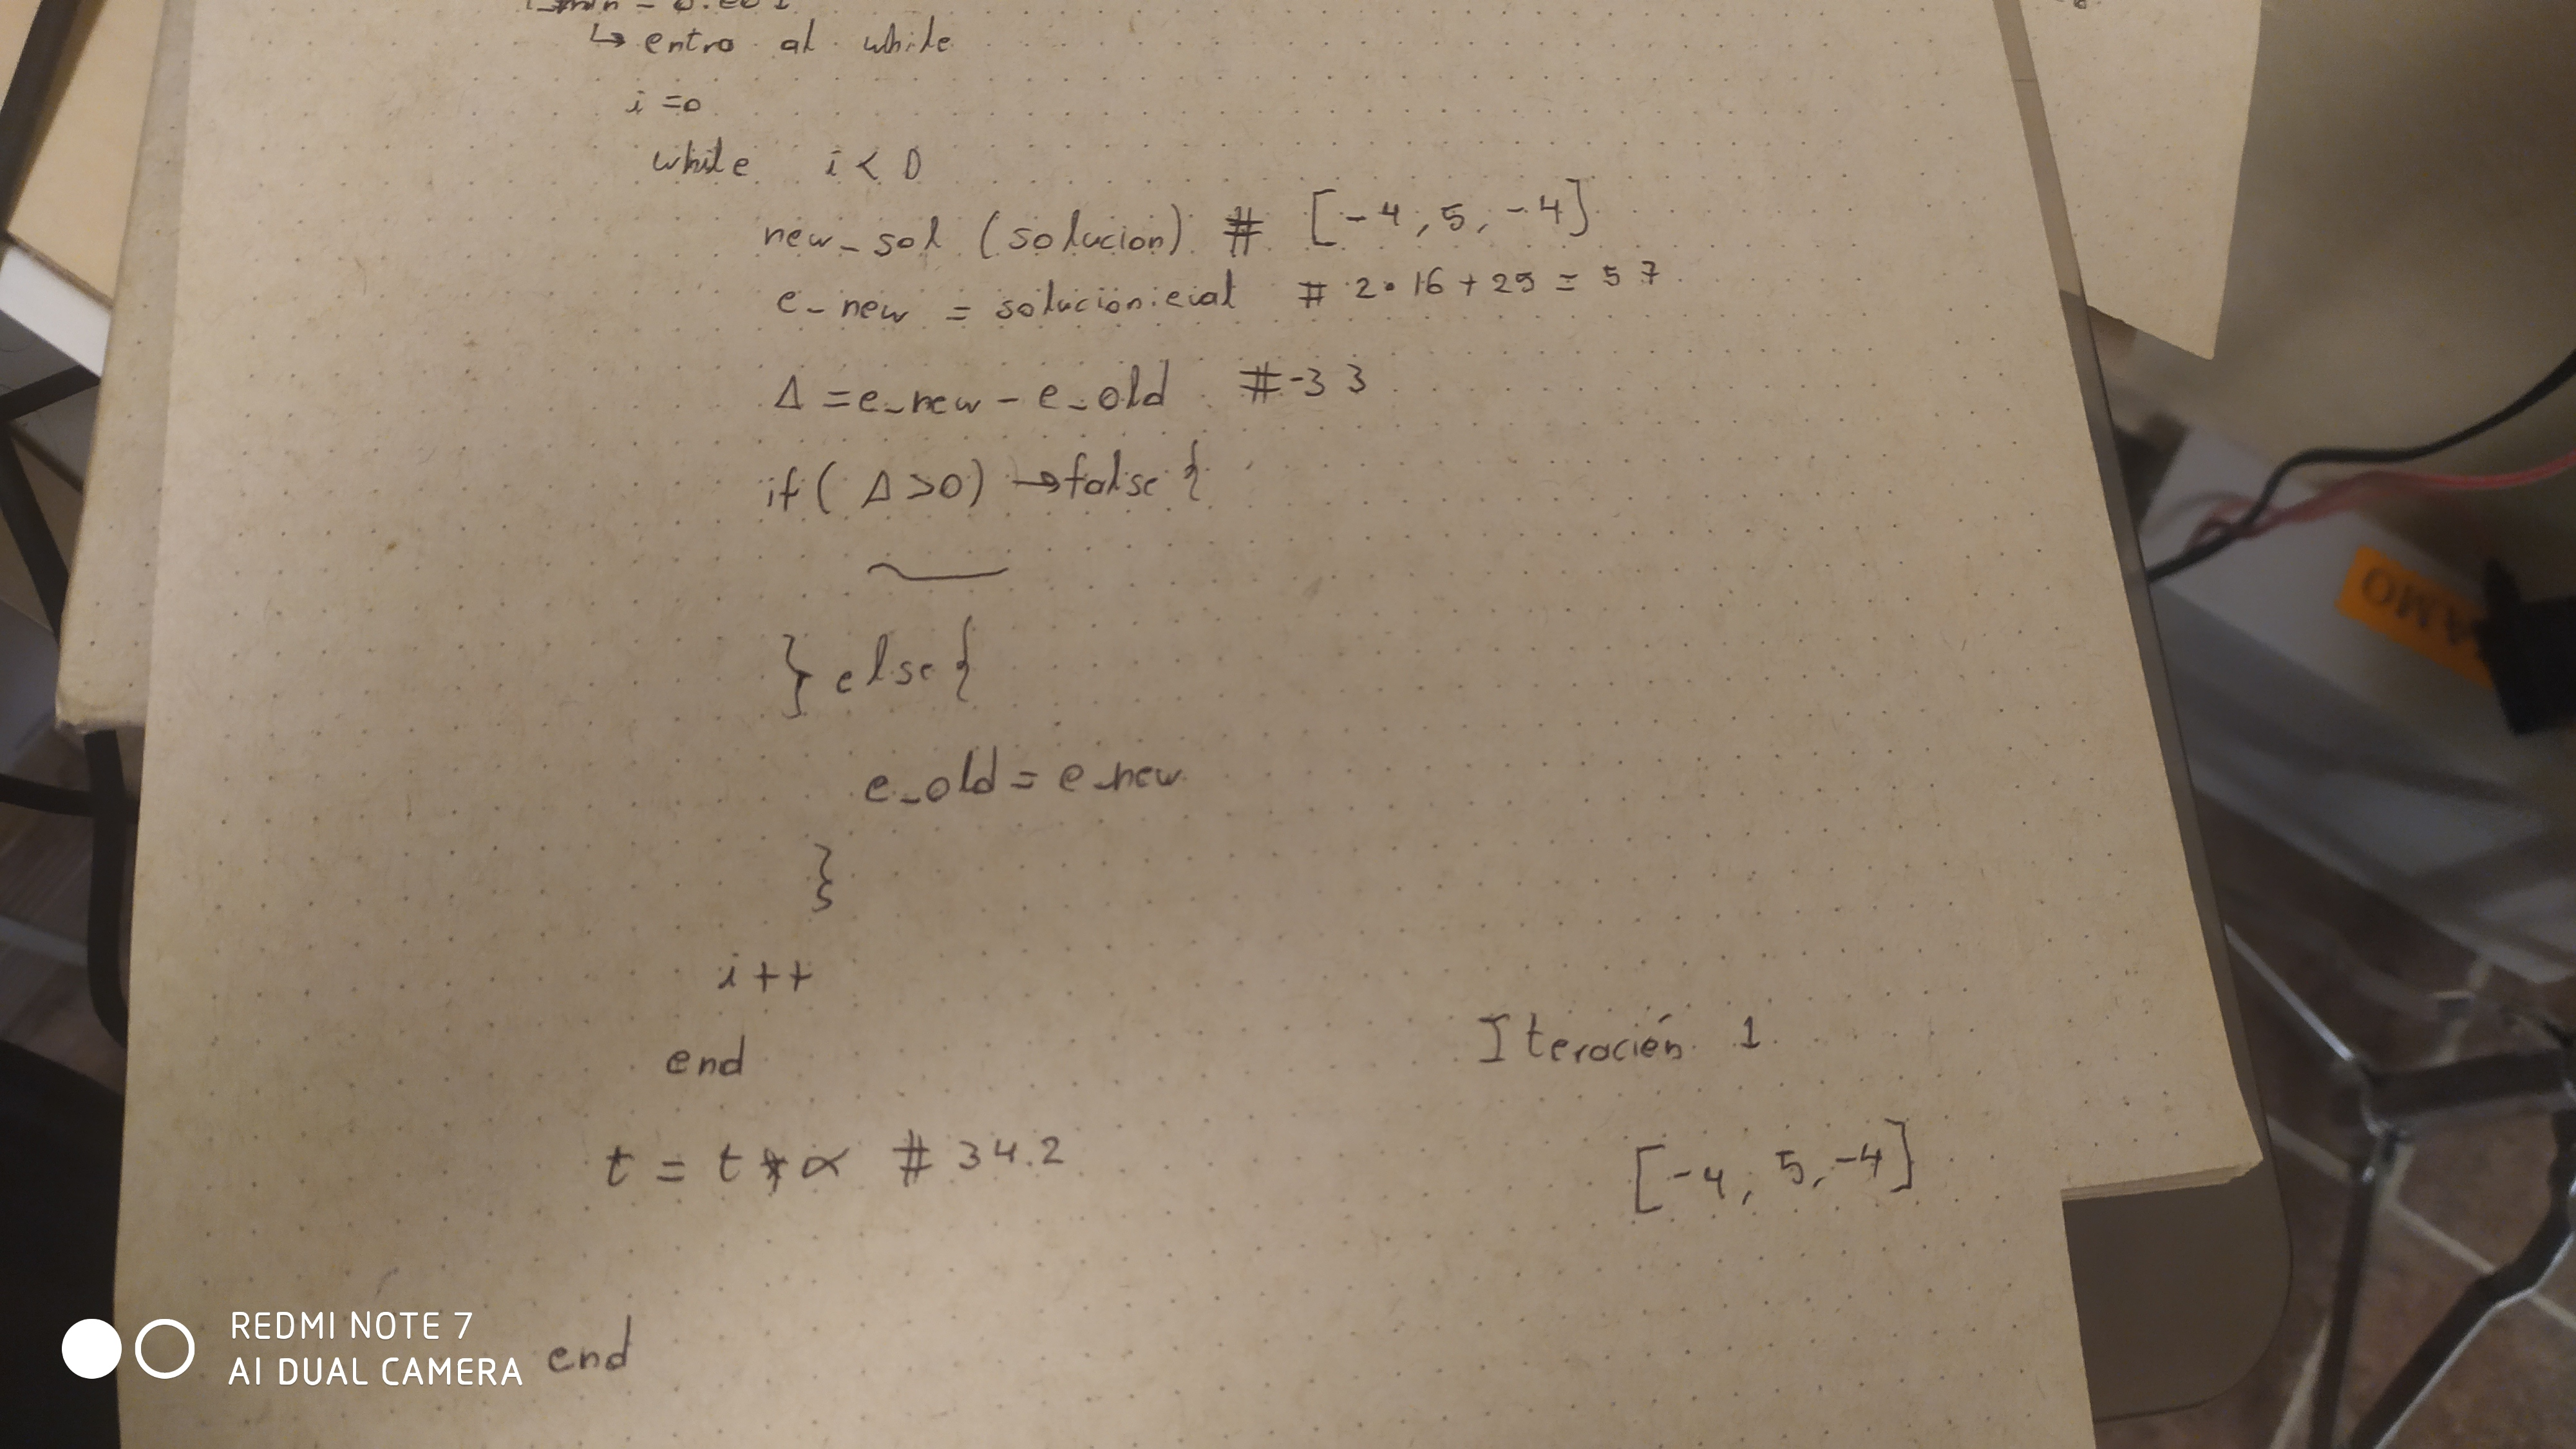
\includegraphics[scale=0.135]{imgs/min-2.jpg}

\end{document}
